\documentclass[a4paper,11pt]{report}

\usepackage[utf8]{inputenc}
\usepackage{ulem}
\usepackage[frenchb]{babel}
\usepackage{graphicx}
\usepackage{listings}
\usepackage{color}
\usepackage{url}
\usepackage{latexsym}
\usepackage{amssymb}
\usepackage{verbatim}
\usepackage{xargs}
\usepackage{float}
\usepackage{vmargin}
\usepackage[pdfborder=RadiusH]{hyperref}
\setmarginsrb{3cm}{2cm}{3cm}{2cm}{0cm}{2cm}{0cm}{2cm}


\definecolor{colKeys}{rgb}{0,0,1}
\definecolor{colIdentifier}{rgb}{0,0,0}
\definecolor{colComments}{rgb}{0,0.5,1}
\definecolor{colString}{rgb}{0.6,0.1,0.1}

%\newcommandx*\image[3][1=., 2=0.8]{\begin{figure}[H]\begin{center}\includegraphics[width=#2\textwidth]{#3}\caption{#1}\end{center}\end{figure}}
\newcommandx*\image[3][1=., 2=1]{\begin{figure}[h!]\begin{center}\includegraphics[width=#2\textwidth]{#3}\caption{#1}\end{center}\end{figure}}
%\newcommandx*\image[3][1=., 2=1]{#1 #2 $#3$\\}
%\newcommand{\image}[2][1]{\begin{center}\includegraphics[width=#1\textwidth]{#2}\end{center}}
%\newcommand{\image}[2][1]{\begin{center}$#2$\end{center}}


\begin{document}
\title{Étude du GMRES dans un code de simulation de réservoir}
\author{Corentin Rossignon\\
  Encadrants INRIA : Olivier Aumage, Samuel Thibault\\
  Encadrant TOTAL : Pascal Hénon}
\date{Février - Août 2011}
\maketitle

\tableofcontents

% R: Ok, O:
\chapter*{Introduction}
 La simulation physique est un élément essentiel de nos jours pour
 comprendre le monde qui nous entoure. Elle est utilisée aussi bien
 pour prédire le temps que pour réaliser des essaies nucléaires sans
 impact radioactif sur l'environnement. Ces simulations sont gourmandes en
 puissance de calcul et doivent souvent s'exécuter plus vite que dans
 la nature ; par exemple : mettre deux jours à calculer le temps du
 lendemain n'est pas intéressant. Les machines réalisant ces calculs
 doivent donc être de plus en plus puissantes pour pouvoir donner un
 résultat plus vite et plus précis.

 La première solution utilisée jusqu'aux environs de 
 2005 était d'augmenter la fréquence des processeurs. Cependant, une limite physique
 a été atteinte autour de 4 Ghz, au-delà la dissipation thermique
 n'est plus possible. La
 seconde solution fut d'augmenter le nombre de processeurs.
 L'inconvénient de cette solution est que le programmeur doit changer
 sa façon de programmer et souvent il n'arrive pas, ou ne peut pas, utiliser toute
 la puissance de la machine.

 Dernièrement, la programmation
 GPGPU (General-Purpose Computation on Graphics Hardware) a été proposée,
 elle consiste à utiliser la carte graphique (Graphics Processing Unit
 ou GPU) pour effectuer les
 calculs. Dans certains cas le temps de calcul peut être
 divisé par 100, mais ici aussi, le programmeur doit programmer
 différemment avec de nouvelles contraintes mémoires. 

 Au vu des performances que peut apporter l'utilisation d'un GPU, la
 société Total, dont les activités se concentrent autour de
 l'extraction du pétrole brut et de son raffinage, propose d'accélérer
 leurs simulations en utilisant une solution GPGPU.

 Parmi ces simulations, il existe
 la simulation de réservoir qui est un élément important dans l’étude des
 champs pétrolifères, elle peut couvrir une période de trente ans.
 Actuellement cette simulation est faite sur CPU.
 Ce mémoire propose donc d'étudier l'accélération que l'utilisation
 hybride GPU - CPU peut apporter par rapport à une solution CPU multi-coeur.
 
\chapter{Contexte}
 % R: Ok, O:
 \section{Simulation de réservoir}
  La simulation de réservoir permet d’optimiser le placement
  des puits pour l'extraction du pétrole. Dans cette simulation, le
  temps est discrétisé avec un pas de l'ordre de la journée. Pour
  chaque pas, il est nécessaire de faire converger un système
  non-linéaire, pour cela de nombreux systèmes linaires creux doivent
  être résolus. Les méthodes de résolution de systèmes linaires creux
  utilisent des matrices.

  Les matrices utilisées
  pour cette simulation sont particulières, elles sont creuses
  et sont composées de blocs carrés non nuls positionnés sur des
  diagonales.
  
  \image[Matrices utilisées pour la simulation de réservoir.]{images/matrices_reservoir.pdf}

 % R: Ok, O:
 \section{Les matrices creuses}
  Les matrices creuses sont des matrices essentiellement composées de zéros,
  cette propriété peut être utilisée pour réduire son empreinte
  mémoire ainsi que le nombre
  d'opérations effectuées lors de l'utilisation d'une telle matrice.
  Pour le cas du produit matrice/vecteur creux, aussi appelé SpMV, le
  nombre de multiplication et d'addition est réduit.

   \begin{figure}[h!]\begin{center}
     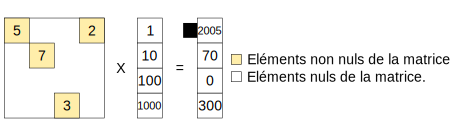
\includegraphics[width=0.8\textwidth]{images/spmv.pdf}
     \label{spmv_sample}
     \caption{Multiplication matrice/vecteur creux - SpMV.}
   \end{center}\end{figure}

  Dans cet exemple (voir figure \ref{spmv_sample}), seules 4 multiplications et 4 additions sont
  nécessaires au lieu des 16 multiplications et 16 additions que nous
  aurions effectuées dans un cas de même taille dense.
  
  Pour ne pas avoir à stocker tous les zéros, seuls les éléments non
  nuls (NZ) sont stockés. Différents formats de stockage de matrices
  creuses existent comme le COO ou le CSR.
  Le format a un impact sur la taille de la matrice en mémoire et sur
  l'ordre des accès mémoires.

 % R: Ok, O:
 \section{Les méthodes itératives}
  Il existe plusieurs méthodes de résolution de systèmes linéaires
  creux, dont les méthodes itératives font partie. L'idée principale de
  ces méthodes est de faire converger la solution en effectuant de
  nombreux SpMV\cite{Saad96IMSLS}. Il est aussi possible de
  préconditionner la matrice pour diminuer le nombre de SpMV à faire.
  
  La méthode ILUk, par exemple, consiste à factoriser partiellement la
  matrice (A) en deux matrices triangulaires : une inférieure (L) et une supérieure
  (U).
  \image[Résolution de $Ax=b$ par une méthode ILUk itérative][0.7]{images/decompo_lu.pdf}
  Puis pour résoudre $Ax=b$, il faut résoudre $Ly=b$ et $Ux=y$ mais comme la
  matrice n'était que partiellement factorisée, nous devons réitérer
  les résolutions L et U pour faire converger $x$ vers la solution
  finale. Le GMRES, que nous détaillerons plus tard, est une méthode
  itérative.

 % R: Ok, O:
 \section{La programmation GPGPU}
  La programmation GPGPU consiste à détourner l'utilisation du
  processeur graphique (GPU), qui habituellement effectue des calculs
  liés à l'affichage, pour lui faire effectuer des calculs
  généralistes. Pour cela, nous devons écrire 
  un code, aussi appelé \textit{Kernel}, dans un langage exprimant le
  parallélisme (CUDA \cite{cuda11} pour une carte NVIDIA ou OpenCL
  \cite{opencl10} pour la portabilité). Dans ces langages, le
  parallélisme est exprimé sous la forme de Thread, un Thread
  représente une instance du \textit{Kernel} auquel on a donné un identifiant.
  Les Threads sont organisés en groupes appelés Warp, les Threads
  d'un même Warp sont totalement synchrones. Pour CUDA la taille d'un
  Warp est de 32. Les Threads sont répartis
  dans des blocs (\textit{Block}) et ces blocs sont eux-mêmes répartis dans une
  grille (\textit{Grid}). La taille des blocs et de la grille déterminent le
  nombre de Threads. Par exemple, si nous avons 512 Threads par bloc et
  512 blocs dans la grille, alors nous aurons un total de 262144 Threads.
  
  \image[Organisation des Threads pour la programmation GPGPU.][0.5]{images/decoupage_cuda.pdf}
  Dans CUDA, l'appel des fonctions GPU et la gestion des identifiants
  se font de la manière suivante:

  \begin{figure}[H]\begin{center}\verbatiminput{exemple.cu}\caption{Exemple de code CUDA}\end{center}\end{figure}

  L'identifiant local correspond à l'identifiant d'un Thread à
  l'intérieur d'un bloc, il est donc compris entre 0 et
  511. Plusieurs Threads dans des blocs différents peuvent avoir le
  même identifiant local. L'identifiant global est unique à chaque Thread.

  \image[Comparaison architecture CPU - GPU.]{images/compar_cpu_gpu.pdf}
  
  Le GPU, à l'inverse du CPU, est surtout composé d'unités de calcul.
  Cela permet de pouvoir faire s'exécuter un grand nombre de Threads en
  parallèle. Regardons plus en détail l'architecture des unités de
  calcul du GPU :
  
  \image[Architecture d'un Streaming Processor.]{images/streaming_processor.pdf}
  
  Le GPU est composé d'unités SIMD appelées Streaming Processor (SP), ces
  unités sont capable à un instant T d'exécuter N instructions
  identiques sur N données potentiellement différentes, avec N la
  taille d'un Warp. En revanche, si un Thread du Warp suit
  un branchement différent des autres, alors il faudra 2 cycles pour
  exécuter les N instructions.

  Il existe deux types de mémoire sur
  GPU :
  \begin{itemize}
  \item la mémoire partagée (\textit{shared memory}), de petite taille et avec une faible
    latence partagée entre les Threads d'un bloc.
  \item la mémoire globale (\textit{global memory}), commune à tous les Threads, mais avec une
    latence élevée qui peut être masquée par l'utilisation
    d'un grand nombre de Threads.
  \end{itemize}

  Les accès à
  la mémoire globale présentent une contrainte, pour que les 32
  instructions puissent s'exécuter en parallèle, les 32 données doivent
  être présentes dans le SP, or la mémoire globale ne peut envoyer que 128 octets à
  la fois (soit 32 float), les Threads doivent donc accéder aux données contiguës en
  mémoire, ce que l'on nomme faire des accès coalescés. Si les données sont
  réutilisées plusieurs fois, il peut être avantageux de les placer
  dans la mémoire locale (\textit{shared memory}) pour minimiser la latence et aussi pour pouvoir faire
  des accès désordonnés à la mémoire locale plutôt qu'à la mémoire globale.

 % R: Ok, O:
 \section{StarPU}
  StarPU\cite{AugThiNamWac11CCPE} est un support exécutif développé par
  l'INRIA et le LaBRI. Il fournit un modèle d’exécution unifié pour les machines
  multi-coeurs équipées d'accélérateurs afin d’exploiter l’intégralité
  de la puissance de calcul tout en s’affranchissant des difficultés
  liées à la gestion des données.
  
  L'application doit enregistrer ses données auprès de StarPU qui en
  interne utilise une DSM (Distributed Shared Memory) réalisant de
  manière transparente les transferts mémoires entre les unités de calcul.

  Puis, l'application crée des tâches décrivant pour
  chaque unité de calcul un code spécifique ainsi que les données
  nécessaires. 

  StarPU s'occupera ensuite d'ordonnancer les tâches sur
  les différentes unités de calcul en prenant en compte le temps des
  transferts mémoires et le temps de calcul.

 % R: Ok, O:
 \section{Solutions existantes de SpMV}
  Lors de mes recherches sur les solutions existantes de SpMV sur GPU,
  deux solutions se sont détachées du groupe : Cusparse et Cusp. Elles
  utilisent toutes les deux CUDA.
  
 % R: Ok, O:
  \subsection{Cusparse}
   Cusparse\cite{cusparse11} est une bibliothèque développée par NVIDIA et distribuée
   avec le SDK de CUDA. Cette bibliothèque fournit quelques opérations
   de bases d'algèbre linéaire creuse, tel que le SpMV et le SpMM
   (produit matrice/matrice creux) pour
   la catégorie BLAS 2 et BLAS 3. Les BLAS sont des routines
   d'algèbres linéaires.

   En ce qui concerne le SpMV, les matrices sont stockées au format
   CSR. Plus loin, dans les tests, nous verrons que le format CSR n'est
   pas le format le plus approprié au SpMV sur GPU.
   
 % R: Ok, O:
  \subsection{Cusp}
   Cusp\cite{Cusp}\cite{BeGa08cusp} est une bibliothèque sous licence Apache 2.0,
   implémentant diverses opérations d'algèbre linéaire creux, dont le
   SpMV, sur GPU et CPU. Cette bibliothèque est générique ( le type
   des coefficients des matrices sont paramétrables ) et
   performante. Elle propose différents formats de stockage
   des matrices, tel que COO, CSR, DIA, ELL et un format hybride
   ELL+COO. Son seul
   inconvénient est que dans le cas d'une machine multi-GPU,
   elle ne permet pas d'utiliser tous les GPU en même
   temps\cite{cuspNoMulti}.

   Pour notre problème, StarPU doit pouvoir
   gérer lui-même la mémoire. Or, Cusp ne nous laisse
   pas la gestion des transferts mémoires en plus de ne pas être
   multi-GPU ; il n'est donc pas possible d'utiliser cette bibliothèque
   en même temps que StarPU.
   Malgré cela Cusp est performante dans le cas de
   matrices génériques. C'est pourquoi nous l'utiliserons comme référence de
   performances pour nos \textit{Kernels}.

 % R: Ok, O:
 \section{Proposition}
  Dans un premier temps, nous écrirons un produit matrice/vecteur creux,
  optimisé pour nos matrices, qui utilise à la fois les unités de
  calculs CPU et GPU. Pour cela nous allons découper nos matrices en
  plusieurs morceaux représentant chacun une tâche StarPU,
  ces tâches pourront être ensuite réparties sur les différents coeurs
  de calcul. Pour les unités GPU, nous rechercherons un format adapté à nos
  matrices qui pourra être moins générique mais plus performant que
  les formats utilisés par Cusp.

  Puis, nous élaborerons un algorithme permettant de faire une
  résolution LU sur GPU.

  Et enfin nous couplerons ces deux opérations pour avoir un GMRES
  fonctionnant en partie sur GPU.

  % R: Ok, O:
\chapter{Formats de stockage et performances}
 Le format de stockage des matrices creuses ayant un impact sur les
 performances du SpMV, nous avons essayé de déterminer quel 
 format est le plus performant sur GPU pour nos matrices.

 % R: Ok, O:
 \section{Réalisation des tests}
  La machine de test est composée de 3 Tesla C2050 (puissance de crête :
  1030 Gflops et 3 Go de mémoire pour un GPU) et de 2 Xeon X5650 (6 coeurs,
  2.66 GHz pour un CPU).

  Les résultats sont exprimés en flops, pour chaque élément non nuls
  de la matrice, nous effectuons une multiplication et une addition, la
  formule pour calculer les flops est donc : $(2 * NNZ) / Temps$, NNZ
  représente le nombre d'éléments non nuls.
  
  Les matrices utilisées sont générées par un programme développé par
  Total et sont représentatives de ce qui est réellement utilisé.
  
  Ces matrices représentent un domaine 3D. Pour chaque élément du
  domaine, le nombre de variables de l'élément correspond à la taille
  des blocs de la matrice. La dimension de la matrice est égale à la
  dimension du domaine à la puissance 3. 
  
  Dans les résultats, nous nommerons les matrices de la façon
  suivantes: ``NNZ TailleBloc TailleDimension''.
  
  La taille des matrices choisies correspond à ce
  qui est actuellement utilisé dans la simulation de réservoir. 
  Dans les cas réels, le paramètre TailleBloc varie entre 3 et 21,
  nous avons choisi les valeurs 4, 8, 9 et 16 pour pouvoir évaluer
  l'impact de la taille des blocs sur les performances de chaque
  format. La valeur 9 est particulière car il s'agit d'une valeur qui
  dans le cas du BCSR sur GPU peut donner de mauvaises performances.
  La taille des
  dimensions ne fait qu'augmenter la taille de la matrice, en prenant
  20 et 30 nous aurons à la fois des problèmes de petite taille et
  des problèmes de taille raisonnable. Nous avons aussi rajouté une
  matrice composée de blocs carrés 16x16 et 40 en dimension, ainsi nous
  aurons une matrice de grande taille qui nous permettra d'estimer
  les limites des formats.

 % R: Ok, O:
 \section{SpMV sur CPU}
  Pour pouvoir avoir une référence, nous utilisons la bibliothèque MKL
  d'Intel regroupant des routines d'algèbres linéaires efficaces.
  Nous utiliserons la fonction MKL qui effectue un produit
  matrice/vecteur creux sur une matrice stockée au format CSR.
  
  \image[Résultats du SpMV sur 2 Xeon X5650 de 6 coeurs chacun soit 12 coeurs cadencés à 2.66 GHz.]{resultats/MKL_CSR_CPU.pdf}

  Si nous utilisons un coeur de calcul CPU nous obtenons environ 1
  Gflop. Dans le meilleur cas, avec 12 coeurs de calcul nous
  pourrions espérer avoir 12 Gflops. Cependant, le débit mémoire nous limite à 25
  Go/s (débit théorique : 32 Go/s), ce qui correspond à 5.5 Gflops.
  Par conséquent, augmenter le nombre de CPU serait inutile.

  Nous venons de voir qu'au maximum nous obtenons 5.5 Gflops, ce qui
  reste peu par rapport au 15 Gflops que nous pourrions obtenir sur un
  seul GPU\cite{VOFG10Improving}. Nous décidons donc que pour notre
  problème, le CPU n'est pas assez performant pour aider le GPU. A
  présent, nous travaillerons uniquement sur GPU.

 % R: Ok, O:
 \section{SpMV sur GPU}
  Pour l'implémentation d'un \textit{Kernel} SpMV sur GPU, plusieurs questions
  doivent être posées :
  \begin{itemize}
   \item Combien de Threads doivent être créer?
   \item Comment distribuer le travail entre les Threads?
   \item Les accès mémoires sont-ils coalescés?
  \end{itemize}
  Pour chaque format nous essayerons de trouver la meilleure réponse.
  
  Pour réaliser le SpMV sur plusieurs unités de calcul, nous essayons
  différentes granularités de découpage des matrices :
  \begin{itemize}
   \item 1 partie : dans ce cas la matrice n'est pas découpée, cela nous
     permet de mesurer l'efficacité du SpMV sur un seul GPU.
   \item 3 parties : nous pouvons maintenant distribuer les calculs sur
     chacun de 3 GPUs et mesurer si le format peut être découpé efficacement.
   \item 9 parties : nous créons un peu plus de tâche que de GPU, cela
     nous permet de voir si le surcoût du découpage n'est pas trop
     important pour pouvoir avoir des tâches plus petites pour que
     StarPU puisse les ordonnancer efficacement sur des GPUs hétérogènes.
   \item 30 parties : nous avons 10 fois plus de tâches que de GPU,
     nous pouvons voir si le format fonctionne aussi bien sur un petit
     ensemble de données pour les mêmes raisons que 9 parties.
  \end{itemize}

  Les tests suivants ont été réalisés en simple précision.

 % R: Ok, O:
 \section[CSR : Compressed Sparse Row]{Compressed Sparse Row}
  \subsection{Analyse du format}
   \image[Compressed Sparse Row.]{images/CSR.pdf}
   
   Les éléments non nuls sont stockés par ligne (NZ), pour chaque élément nous
   avons sa colonne (COL) et sa ligne doit être calculée en utilisant
   PTR. Le tableau PTR correspond à l'indice dans NZ du premier élément
   d'une ligne.
   
  \subsection{Implémentation sur GPU}
   Les Threads peuvent être distribués de deux manières : 1 Thread par
   ligne ou 1 Warp (32 Threads) par ligne. La solution d'un Thread par
   ligne ne permet pas d'avoir des accès mémoires coalescés à NZ et
   COL, et donc produit de très mauvaises performances. A l'inverse, la
   solution du Warp par ligne permet d'avoir des accès mémoires
   coalescés à NZ et COL, mais oblige une réduction du résultat des 32 Threads à la
   fin du calcul qui peut être fait efficacement avec la technique de
   Mark Harris\cite{HarrisReductionCUDA}. Comme l'algorithme
   fonctionne par ligne, la matrice peut être découpée en nombre égal
   de lignes. Le vecteur multiplicatif doit être transmis à chaque
   unité de calcul et le vecteur résultat est découpé comme la matrice.
   Quelque soit la méthode utilisée, l'ordre des accès au vecteur
   multiplicatif reste indéfini.
   
   \image[Répartition des Threads dans le format CSR.][1]{images/distrib_csr.pdf}

  \subsection{Résultats}
   \image[Résultats du SpMV pour le format CSR.]{resultats/CSR.pdf}
   
   Nous pouvons remarquer que la taille des blocs de la matrice est un
   facteur important, cela vient des accès mémoires, une taille de blocs
   se rapprochant d'un multiple de 32 permet d'augmenter le nombre
   d'accès coalescés au vecteur multiplicatif. Les blocs ayant un
   impact sur le format, nous essayerons plus tard le format BCSR qui
   utilise des blocs plutôt que des coefficients.

   Le nombre de découpages
   n'a pas un fort impact sur les performances car il n'y a aucune
   dépendance entre les morceaux du vecteur résultat. Il suffit juste de
   recoller les bouts. Les résultats mono GPU sont aussi bons qu'avec
   Cusp. Nous obtenons un speed-up de 2.8 en utilisant 3 GPUs, ce qui
   montre que ce format se découpe bien. 

 % R: Ok, O:
 \section[DIA : Diagonal format]{Diagonal format}
  \subsection{Analyse du format}
  \image[Diagonal format.]{images/DIA.pdf}
  
   Le format DIA tient compte de la structure de la matrice, si les
   éléments non nuls de la matrice sont concentrés sur des
   diagonales, ce qui est le cas dans les matrices que nous voulons
   manipuler, alors il suffit de stocker toutes les diagonales qui
   contiennent un éléments non nul en remplissant le vide par des zéros et
   dans un autre tableau, stocker le numéro de la diagonale, les
   nombres négatifs correspondent aux diagonales basses, les positifs
   aux diagonales hautes, le 0 à la diagonale centrale. Grâce au numéro
   de diagonale, nous pouvons retrouver la taille de la
   diagonale ($nx-|diag|$).

  \subsection{Implémentation sur GPU}
   Comme pour le CSR nous avons plusieurs choix de distribution; 4
   au total, 1 Thread/Warp par ligne/diagonale. Toutes les solutions
   de distribution par diagonale impliquent soit d'avoir un vecteur
   résultat temporaire par Thread/Warp soit d'effectuer des écritures
   atomiques, ces deux solutions sont peu performantes voir
   impossibles. En attribuant un Thread à une ligne, et grâce à la
   synchronisation du Warp, nous sommes sûrs que tous les Threads d'un Warp
   travaillent sur la même diagonale et accèdent donc de manière
   coalescer et directe à NZ et au vecteur multiplicatif.
   
   \image[Répartition des Threads dans le format DIA.]{images/distrib_dia.pdf}
   
   Toutefois, cette
   solution comporte un problème sur les bords de la matrice, il y
   aura des Threads qui n'auront rien à faire, par exemple pour la
   diagonale -31, seul le Thread 32 aura une opération à effectuer,
   les 31 autres Threads (1-31) attendront.

  \subsection{Résultats}
   \image[Résultats du SpMV pour le format DIA classique.]{resultats/DIA.pdf}
    
    Si nous comparons nos résultats avec ceux de Cusp, qui sont
    environ 10 Gflops supérieurs, nous pouvons voir que nous
    n'obtenons pas un résultat optimal. Le problème provient du stockage
    de la matrice. En effet, au lieu de stocker des diagonales avec différentes
    tailles, nous devrions normaliser leurs tailles pour permettre au
    GPU de trouver plus facilement une diagonale, cela évite l'utilisation
    d'un tableau d'indirection qui était coûteux. De plus, la normalisation des
    diagonales n'augmente que la taille en mémoire de la matrice sans changer
    le nombre d'opérations à effectuer.
   
    \image[Résultats du SpMV pour le format DIA orienté GPU.]{resultats/DIA_improved.pdf}
    
    Les résultats sont meilleurs et concordent avec Cusp. Cependant la
    structure de nos matrices n'est pas optimale pour cette version
    du DIA, cela provient du fait qu'elles sont blocs-diagonales. Le
    problème apparaît pour les diagonales du bord des blocs, car ces
    diagonales se retrouvent avec plus de zéro que d'éléments non
    nuls.

    \image[Zoom sur le problème de remplissage d'une diagonale.][0.6]{images/dia_fill.pdf}
    
    Pour résoudre ce problème, il faudrait créer un nouveau format qui
    serait un DIA par bloc.

 % R: Ok, O:
 \section[ELL : ELLPACK format]{ELLPACK format}
  \subsection{Analyse du format}
   \image[ELLPACK format.]{images/ELL.pdf}
   
   Le ELL consiste d'abord à ``pousser'' tous les éléments vers la gauche,
   puis à remplir de zéros pour créer une structure rectangulaire. Pour
   chaque élément nous enregistrons sa colonne dans COL (ou -1 pour les
   zéros). Ce format peut être stocké soit au format \textit{row major} (les données contiguës
   appartiennent à la même ligne), soit au format \textit{column major} (les données contiguës
   appartiennent à la même colonne).

  \subsection{Implémentation sur GPU}
   La première question à se poser concerne l'ordre de stockage de la
   matrice. Le \textit{row major} revient à avoir un CSR avec des zéros
   supplémentaires, alors que le \textit{column major} nous offre plus de
   parallélisme en permettant d'avoir un Thread
   par ligne tout en gardant des accès coalescés à NZ.
   
   \image[Répartition des Threads dans le format ELL.][1]{images/distrib_ell.pdf}

  \subsection{Résultats}
   \begin{figure}[h!]\begin{center}
     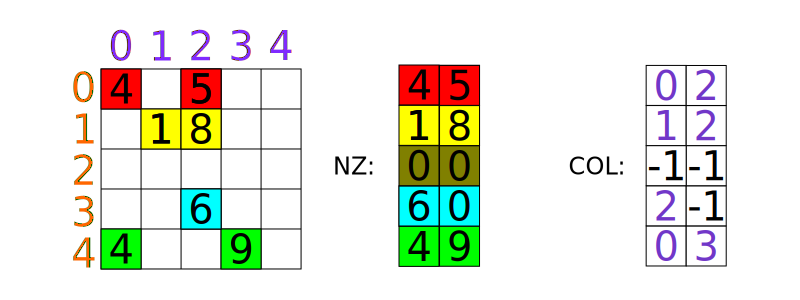
\includegraphics[width=0.8\textwidth]{resultats/ELL.pdf}
     \caption{Résultats du SpMV pour le format ELL en \textit{column major}.}
     \label{res_ell}
   \end{center}\end{figure}
   
   Les résultats sont plutôts bons car nous travaillons sur des matrices
   régulières, il n'y a donc quasiment pas d'ajout de zéros. De plus, grâce
   à la structure en bloc de nos matrices, les accès au vecteur
   multiplicatif se retrouvent mutualisés. Les performances sont aussi
   bonnes que Cusp.

 % R: Ok, O:
 \section[JAD : JAgged Diagonale storage]{Jagged Diagonal Storage}
  \subsection{Analyse du format}
   
   Le JAD est un format dérivé du ELL, pour éviter l'ajout de
   zéros les lignes sont réordonnées par taille et les permutations
   sont stockées dans PERM. Le vecteur final s'obtient en appliquant
   PERM au vecteur résultat.

  \subsection{Implémentation sur GPU}
   Le JAD étant un dérivé du ELL, les problématiques de l'implémentation
   sont les mêmes que pour le ELL, nous avons donc un Thread par ligne.
   
  \subsection{Résultats}  
   Les résultats (voir figure \ref{res_jad}) sont aussi bons que ceux du format ELL. Cependant, le
   JAD peut se montrer plus performant que le ELL dans le cas de
   matrices non régulières, mais ce n'est pas notre cas.
   
   Cusp n'implémente pas le format JAD. En contrepartie, un format
   hybride ELL+COO est utilisé pour les matrices non régulières.

   \image[JAgged Diagonale storage.]{images/JAD.pdf}
   \image[Répartition des Threads dans le format JAD.][1]{images/distrib_jad.pdf}
   \begin{figure}[h!]\begin{center}
     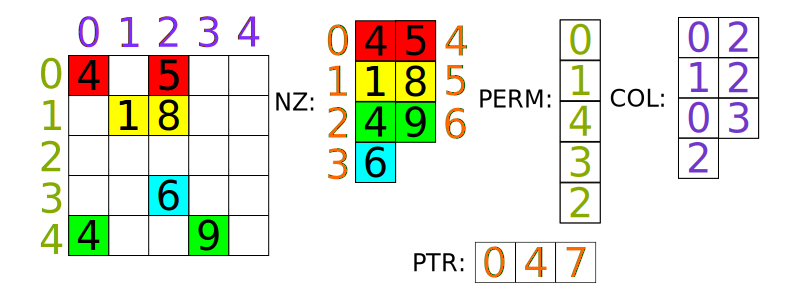
\includegraphics[width=0.8\textwidth]{resultats/JAD.pdf}
     \caption{Résultats du SpMV pour le format JAD.}
     \label{res_jad}
   \end{center}\end{figure}


 % R: , O:
 \section[BCSR : Block Compress Sparse Row]{Block Compress Sparse Row}
  \subsection{Analyse du format}
   \image[Block Compress Sparse Row. Taille des blocs = 2.]{images/BCSR.pdf}
   
   Le BCSR reprend le principe du CSR mais stocke des blocs. Pour
   minimiser l'ajout de zéros, nous avons des blocs à une dimension, ce
   qui correspond à regrouper des lignes. A l'intérieur des blocs, les
   données peuvent être stockées soit en \textit{column major} soit en \textit{row major}.

  \subsection{Implémentation sur GPU}
   Le premier choix d'implémentation consiste à choisir un Thread par
   bloc ou un Warp par bloc. Le choix du Warp permet d'exploiter le
   parallélisme offert par les blocs, mais impose une limitation. Pour
   que les Threads n'effectuent qu'une seule réduction, ils doivent
   rester sur la même ligne durant le calcul d'un bloc, ce qui oblige
   à avoir un diviseur de 32 comme taille de bloc.
   
   \image[Répartition des Threads dans le format BCSR.]{images/distrib_bcsr.pdf}

   Dans le cas où le BCSR est constitué de blocs dont la taille n'est
   pas un diviseur de 32, par exemple 3, la
   répartition du Warp dans le bloc pose problème et oblige
   l'utilisation pour chaque thread d'un tableau temporaire sur lequel
   une réduction sera faite à la fin.

   Ensuite nous devons choisir la taille des blocs, celle-ci dépendant
   de la taille des blocs en entrée et ne pouvant pas se calculer,
   nous essayerons dans le Chapitre \ref{BCSR_bloc_size} différentes
   tailles de blocs.
   
  \subsection{Résultats}
   Les résultats sur les figures \ref{res_bcsr_row} et \ref{res_bcsr_col} ont été obtenus avec des blocs BCSR de taille 8.
   
   \begin{figure}[h!]\begin{center}
     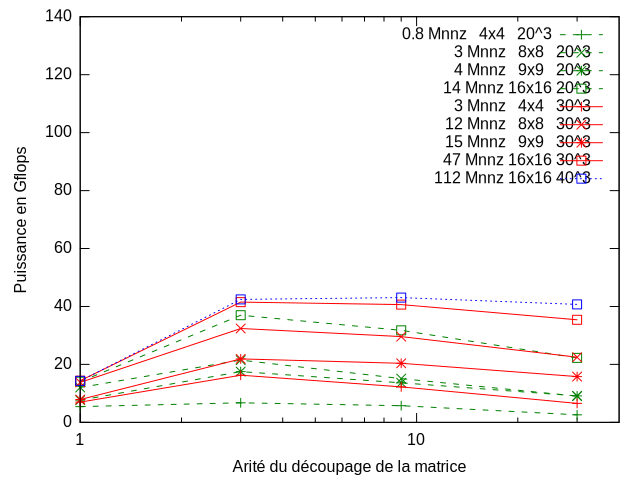
\includegraphics[width=0.8\textwidth]{resultats/BCSR_row.pdf}
     \caption{Résultats du SpMV pour le format BCSR en \textit{row major}.}
     \label{res_bcsr_row}
   \end{center}\end{figure}
   \begin{figure}[h!]\begin{center}
     \includegraphics[width=0.8\textwidth]{resultats/BCSR_col.pdf}
     \caption{Résultats du SpMV pour le format BCSR en \textit{column major}.}
     \label{res_bcsr_col}
   \end{center}\end{figure}
   
   L'organisation des données \textit{column major} offre de meilleures performances
   qu'en ligne, cela s'explique par le fait que les accès au vecteur
   multiplicatif deviennent mutualisés tout en gardant des accès à NZ
   et COL coalescés. 
   Nous pouvons remarquer que la taille des blocs de la matrice a un
   impact important sur les performances. Dans ce cas, il faut avoir
   une taille de blocs multiple de 8 pour obtenir le maximum de
   performances. Malgré les mauvaises performances obtenues avec les
   blocs 9x9, le BCSR reste très efficace.
   
 % R: Ok, O:
\clearpage
 \section{Format non testés}
  Les formats suivants n'ont pas été testé car leurs implémentations
  sur GPU seraient inefficaces.

  \subsection[COO : Coordinate format]{Coordinate format}
   \image[Coordinate format.]{images/COO.pdf}
   
   Ce format stocke, pour chaque élément non nul (NZ) de la matrice,
   ses coordonnées (ROW, COL) ainsi que sa valeur. L'ordre des
   éléments n'étant pas spécifié, il est impossible de savoir où les
   Threads vont écrire. Il faudrait donc créer un vecteur résultat par
   Thread puis faire une réduction sur tous ces vecteurs (utilisation
   coûteuse de la mémoire) ou bien effectuer des opérations atomiques
   sur le vecteur résultat (sérialisation du code).
   
  \subsection[CSC : Compress Sparse Column]{Compress Sparse Column}
   \image[Compress Sparse Column.]{images/CSC.pdf}
   Pour le CSC, les valeurs sont stockées par colonne, à l'inverse du CSR.
   Le problème du portage sur GPU est très proche du problème
   rencontré pour le COO. Ici, il faudrait 1 vecteur par Warp (encore
   trop coûteux) ou alors utiliser des opérations atomiques.

 % R: Ok, O:
 \section{Résumé des performances}
  Le CSR est un format efficace sur CPU mais n'est que relativement
  efficace sur le GPU.

  Le DIA doit être un peu modifié pour le GPU, dans le cas d'une
  matrice composée uniquement de diagonales simples, il se révélera être
  le plus efficace, mais dans notre cas, les blocs induisent un
  surplus de calcul. Un DIA par bloc pourrait résoudre notre problème.

  Le ELL et le JAD sont aussi efficaces sur GPU mais le JAD est à
  privilégier dans le cas d'une matrice non régulière.

  Pour finir, le BCSR \textit{column major} se révèle jusqu'à 1,5x
  plus performant que les autres formats, et même dans le cas d'une
  matrice avec des blocs 9x9 il reste le plus performant.

\chapter{Expérimentation du BCSR}
 \label{BCSR_bloc_size}
 % R: Ok, O:
 L'algorithme actuel du BCSR nécessite des blocs dont la taille est
 une puissance de 2 pour pouvoir être efficace. Or, dans la cas des
 matrices que nous étudions, nous n'aurons pas une puissance de 2 en
 taille de blocs. Nous proposons d'étudier le
 comportement de l'algorithme dans ces cas là. Pour cela nous avons
 généré des matrices dont la taille des blocs est comprise entre 2 et
 32. Pour chaque matrice nous avons choisi un paramètre dimension de
 telle sorte que le nombre d'élément non nuls soit d'environ 27
 Millions.

 Pour chaque matrice nous avons testé deux versions du BCSR en faisant
 varier la taille interne des blocs BCSR parmi 2, 4, 8 et 16.
 
 % R: Ok, O:
 \section{Alignement}
  Si la taille des blocs de la matrice en entrée n'est pas un multiple
  de la taille des blocs BCSR choisi, alors l'algorithme fait du
  remplissage de zéros pour obtenir un bloc BCSR.

  \image[Exemple d'un défaut d'alignement pour une matrice bloc 3 et un BCSR bloc 4]{images/bcsr_align_exp.pdf}
  
  Dans le cas d'une matrice composée de blocs carrés de taille 3 et d'un
  BCSR avec une taille de bloc 4, nous avons un défaut d'alignement
  pour chaque bloc ce qui conduit à presque multiplier par 2 la taille
  de la matrice.
  
  \image[SpMV - BCSR col - 3 GPU - Alignement - 27 Mnnz $\pm$ 1 Mnnz.]{resultats/BCSR_align.pdf}
  
  Lorsque les blocs sont alignés, il n'y a aucun remplissage, par
  contre dans les autres cas il y a remplissage, ce qui conduit à
  augmenter le nombre de calcul.

  Pour un BCSR avec des blocs de taille 8 nous avons un cas
  particulier, si la matrice a des blocs de taille 12 alors le
  remplissage ne se fera qu'une fois sur deux, réduisant ainsi le
  nombre d'opération.

  Quelque soit le nombre de blocs de la matrice, l'utilisation du BCSR
  en bloc 2 donne toujours les plus mauvaises performances alors que
  le BCSR en bloc 8 représente le meilleur compromis.

 % R: Ok, O:
 \section{Remplissage}
  Pour limiter le remplissage, nous rajoutons des lignes de zéros dans
  chaque bloc pour que celui-ci obtienne un nombre de lignes en
  puissance de 2. Cela permet de supprimer le remplissage en $x$ que
  nous avions.
  
  L'ajout de lignes agrandit le vecteur résultat. A la fin du calcul du
  SpMV, nous devrons donc retirer les résultats inutiles du vecteur.

  \image[Exemple d'un remplissage pour une matrice bloc 3 et un BCSR bloc 4.]{images/bcsr_fill_exp.pdf}

  Dans cet exemple notre matrice blocs carrés est transformée en matrice
  avec des blocs 3x4. Nous avons donc minimisé l'ajout de zéros.
  
  \image[SpMV - BCSR col - 3 GPU - Remplissage - 27 Mnnz $\pm$ 1 Mnnz.]{resultats/BCSR_fill.pdf}
  
  Les résultats sont plutôt bons lorsque la taille des blocs de la
  matrice est légèrement inférieure à la puissance de 2 supérieure. Par
  contre si la taille est légèrement supérieure il vaut mieux utiliser
  la méthode du défaut d'alignement.

 % R: , O:
 \section{Limite du BCSR}
  Nous cherchons maintenant les limites du format BCSR, pour cela nous
  choisissons une matrice composée de blocs carrés 16x16 et nous
  faisons varier sa dimension entre 1 et 50.

  \image[SpMV - BCSR col - 3 GPU - Matrice bloc 16 x 16.]{resultats/BCSR_16.pdf}

  Nous obtenons une limite autour de 140 Gflops lorsque nous utilisons
  3 GPUs. Dans les tests que nous avons effectués, le choix d'une
  matrice de dimension 40 nous donne presque les meilleures performances.

 % R: Ok, O:
 \section{Utilisation de GeMV}
  Sur CPU, lorsqu'une matrice creuse comporte des parties denses assez
  grandes, il peut être avantageux d'utiliser une multiplication
  matrice/vecteur dense, ou GeMV, sur les parties denses. Le GeMV est
  un BLAS 2.

  Dans notre cas pour créer des blocs denses, nous devons regrouper les
  blocs d'une même ligne. Il nous faut ensuite construire le vecteur à
  multiplier pour chaque bloc dense.

  Dans le cas où l'on doit exécuter plusieurs SpMV à la suite sur
  une même matrice, la compression de la matrice n'est
  faite qu'une seule fois mais il faut créer à chaque itération autant de
  vecteurs que de GeMV à effectuer. Dans le cas du GPU, il faut
  envoyer ces vecteurs sur le GPU, et faire un appel GeMV pour
  chacun. Or si nous souhaitons utiliser le GeMV fourni par NVIDIA
  dans Cublas, il faut faire les transferts et les appels à GeMV un à
  un.
  
  L'efficacité du calcul ne parvient pas à amortir le coût du
  transfert et des appels.

\chapter{Résolution LU sur GPU}
 La résolution LU consiste à résoudre deux équations $Ly=b$ puis $Ux=y$
 avec L et U deux matrices triangulaires, respectivement basse (\textit{Lower})
 et haute (\textit{Upper}). Pour résoudre une équation avec une matrice
 triangulaire basse, aussi appelé descente, il suffit pour chaque colonne
 de diviser l'élément le plus en haut de la colonne avec l'élément
 correspondant dans $x$ pour obtenir la valeur solution, aussi appelée
 contribution, dans $y$. Avec cette
 contribution nous pouvons soustraire au vecteur $x$ les autres éléments de la colonne
 multipliés par la contribution. Dans le cas d'une matrice creuse, il se
 peut que deux colonnes n'aient pas de contributions entre elles, elles
 peuvent donc être calculées en parallèles.
 
 Les algorithmes de résolution LU multi-CPU actuelles ne permettent pas
 d'exploiter le parallélisme d'un GPU. En effet, dans ces méthodes, la
 distribution du travail consiste à calculer la contribution d'une
 colonne par CPU puis
 libère la possibilité de calculer les contributions d'autres
 colonnes. Sur GPU, calculer les contributions d'une
 colonne ou de plusieurs colonnes coûte quasiment le même temps, nous
 avons donc choisi un algorithme qui fonctionne par étapes. A chaque
 étape, l'algorithme calcule les contributions de toutes les colonnes
 qui n'attendent pas de contributions, jusqu'à ce que toutes les
 contributions de toutes les colonnes soient calculées (fig. \ref{sans_ordering}). En analysant les
 calculs nous pouvons réduire la résolution LU à une suite de TRSV et
 de SpMV, une étape correspondant à un TRSV suivi d'un SpMV.

 \begin{figure}[h!]\begin{center}
     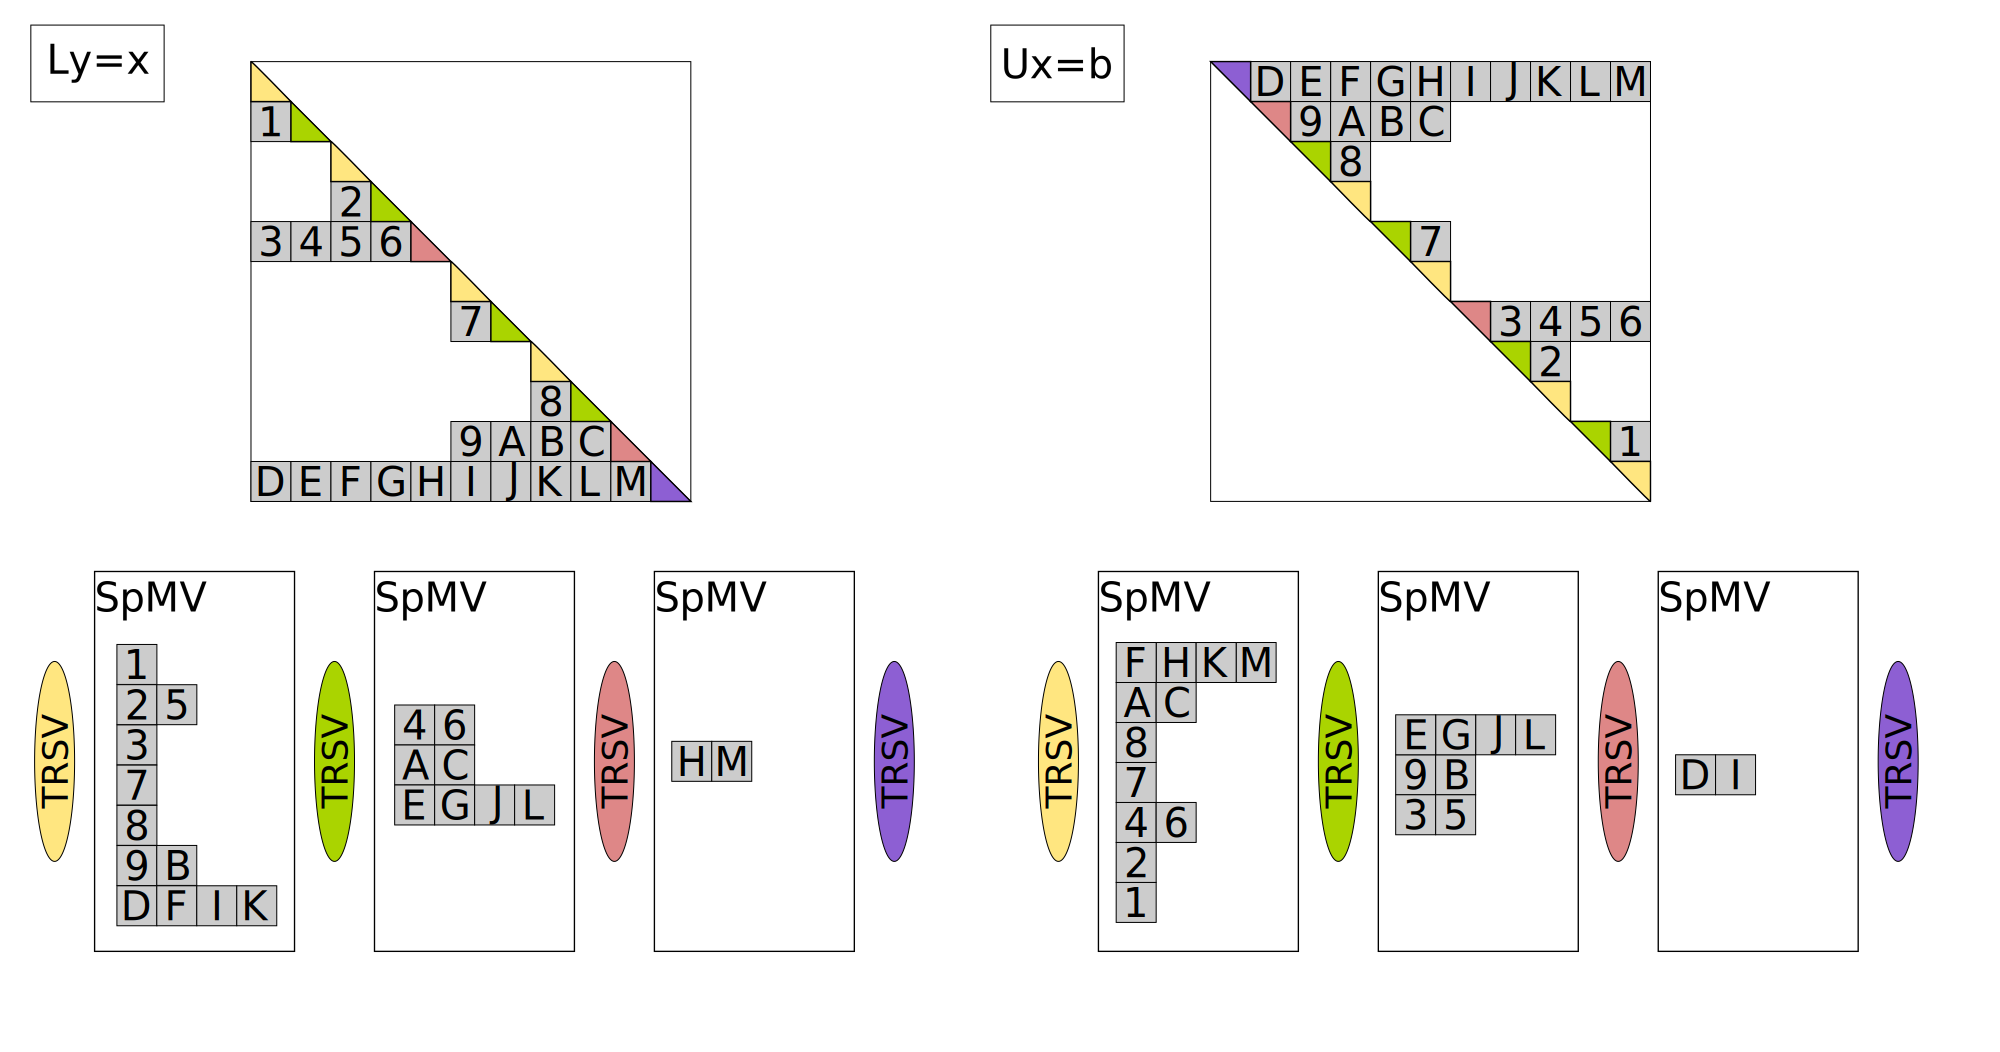
\includegraphics[width=\textwidth]{images_total/LU.pdf}
     \caption{Descente - Remontée d'une matrice sans ordering sur GPU.}
     \label{sans_ordering}
 \end{center}\end{figure}

 Un ordering correspond à une suite de permutations ligne/colonne.
 Le nombre d'étapes dépend de l'ordering utilisé lors de la
 factorisation de la matrice. Une factorisation sans ordering
 spécifique, comme le montre la figure \ref{sans_ordering}, implique
 plusieurs étapes dans l'algorithme. Le choix de l'ordering aura donc un impact
 sur les performances GPU, un plus petit nombre d'étapes implique un
 temps de calcul réduit. L'ordering Rouge-Noir permet de n'avoir qu'une
 seule étape, cf. figure \ref{ordering_rb}, mais augmente le nombre
 d'itérations nécessaire pour faire converger la solution.

 \begin{figure}[h!]\begin{center}
     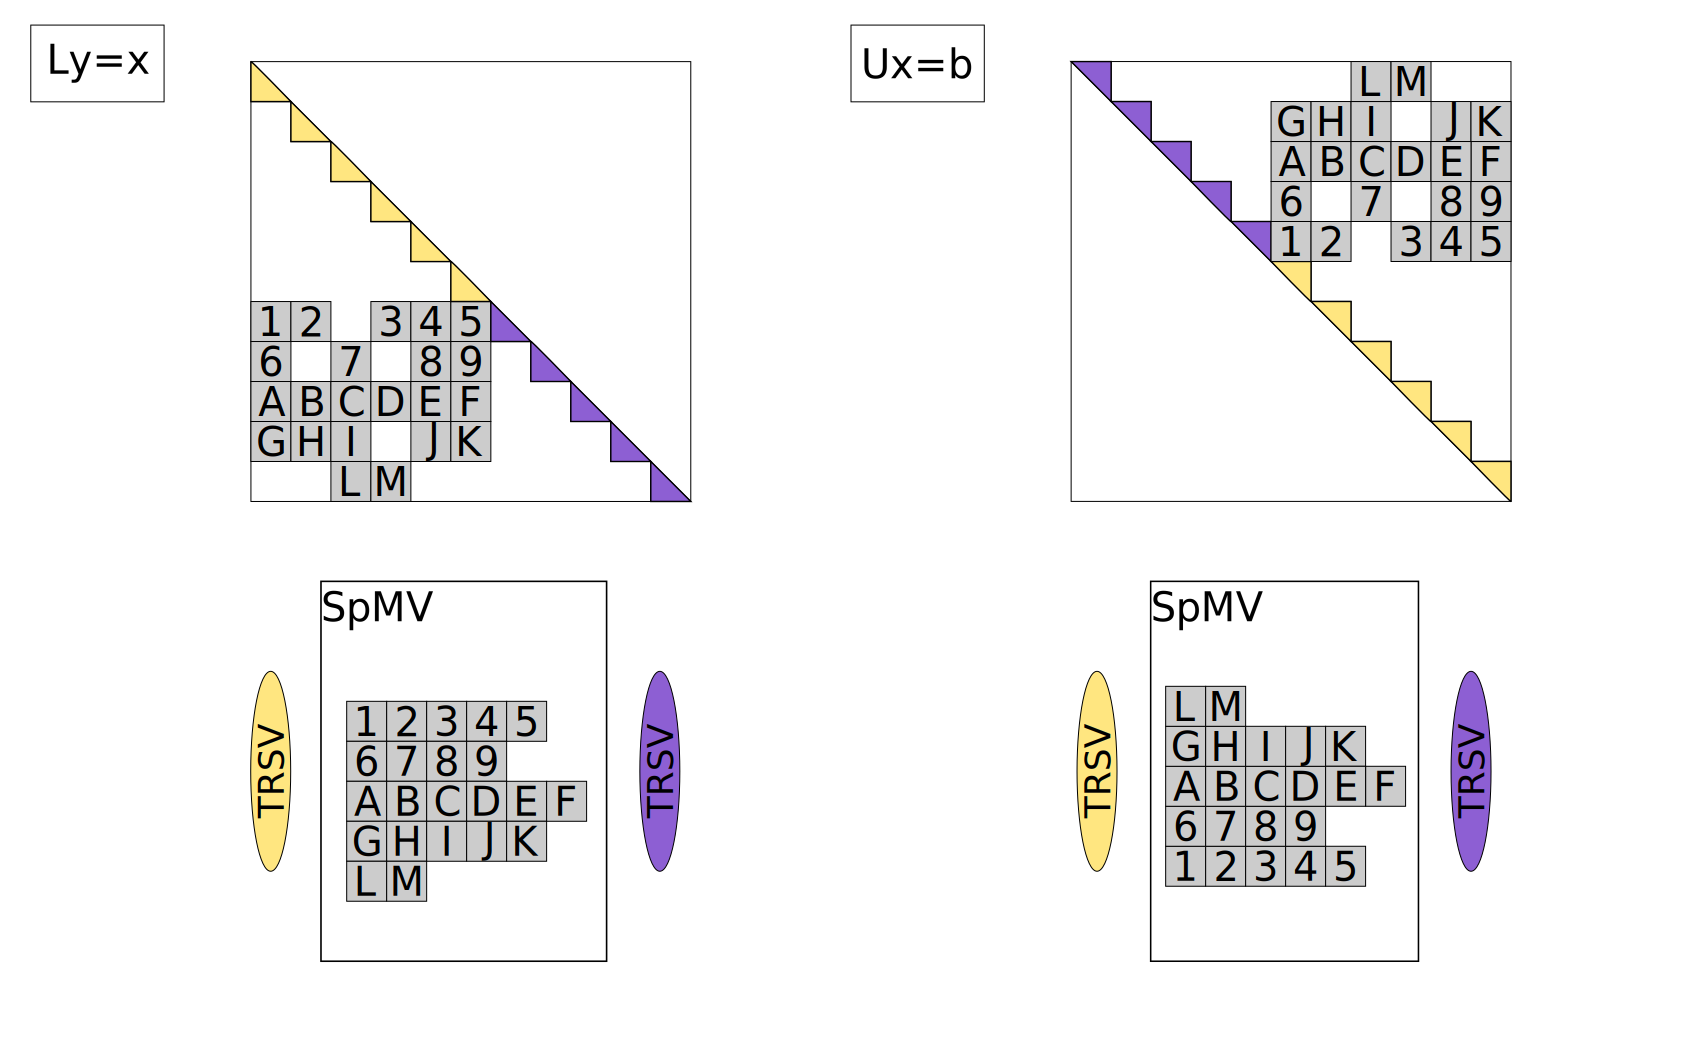
\includegraphics[width=\textwidth]{images_total/LU_improve.pdf}
     \caption{Descente - Remontée d'une matrice avec ordering Rouge-Noir sur GPU.}
     \label{ordering_rb}
 \end{center}\end{figure}
 
 \section{Résultat}
  La machine de test reste la même que pour le SpMV, mais cette fois nous n'utiliserons
  qu'un GPU. Le protocole de test consiste à résoudre une équation
  $Ax=b$ avec $A$ une matrice puis à diviser le temps de la résolution
  par le nombre d'itérations pour connaître le temps moyen d'une itération.
  Les matrices $A$ sont générées
  avec les paramètres TailleDimension = {10, 20, 30, 40} et TailleBloc
  = {1, 4, 8, 16}, ce qui fait un total de 16 matrices.
  
  Les tests suivants ont été réalisés en double précision.
  
  \subsection{GMRES sans ordering spécifique}
   Le nombre d'étapes pour la résolution LU dépend du paramètre TailleDimension:
   \begin{center}
     \begin{tabular}{|c|c|}
       \hline
       TailleDimension & Nombre d'étapes \\
       \hline
       10 & 27 \\
       20 & 57 \\
       30 & 87 \\
       40 & 117 \\
       \hline
     \end{tabular}
   \end{center}
  \image[Temps d'une itération du GMRES sans ordering.]{images_total/none.pdf}
  Sans ordering spécifique, le nombre d'étapes de la résolution LU est
  trop important sur GPU pour concurrencer la version CPU. Dans le
  meilleur cas nous n'obtenons qu'un speed-up de 3.7 et les performances
  sont souvent inférieures à une version mono-CPU.
  
% PRE  % 6.6931112185786175
% RED  % 9.41033306086002



  \subsection{GMRES avec un ordering Rouge-Noir}
   Dans ce cas le nombre d'étapes est égal à 1, les opérations
   effectuées serons donc 2 TSRV et 2 SpMV.
  \image[Temps d'une itération du GMRES avec un ordering Rouge-Noir.]{images_total/red.pdf}
   Nous obtenons un temps d'itération constant, sur les petites
   matrices le CPU est plus efficace mais pour les grandes matrices le
   GPU devient le plus efficace avec un speed-up allant jusqu'à 9.4 .   
  
  \subsection{GMRES sans préconditionneur}
   Si nous n'utilisons pas de préconditionneur, le GMRES ne contient
   qu'un SpMV.
   \image[Temps d'une itération du GMRES sans préconditonneur.]{images_total/pre.pdf}
   Comme nous l'avons vu dans le chapitre précédent le SpMV GPU est
   plus efficace que le SpMV CPU, le GMRES sans préconditionneur est
   donc plus efficace sur GPU que sur CPU. Dans le
   meilleur cas nous obtenons un speed-up de 6.7 .


\chapter{Factorisation LU sur GPU}
 La factorisation LU est une étape difficile à paralléliser sur GPU
 due à son irrégularité de calcul. Mais certaines étapes de la
 factorisation utilisent des BLAS 3 qui peuvent être déchargées sur le
 GPU malgré le coût du transfert mémoire. Nous proposons d'étudier à
 partir le cas du GEMM.
 
 \section{GEMM sur GPU}
  \image[GEMM : Multiplication d'une matrice A par une autre matrice B.]{images_total/GEMM.pdf}
  Lors de la factorisation LU, il peut être intéressant d'utiliser un
  produit matrice/matrice (ou GEMM) lorsque nous avons assez de
  contributions. Le nombre de contributions correspond à la taille M des
  matrices et la taille k correspond à la taille des blocs.
  Le GEMM étant plus efficace sur GPU que sur CPU, nous pouvons espérer
  gagner en performance malgré le
  coût des transferts mémoires entre le GPU et le CPU.
  Nous cherchons pour chaque k compris entre 3 et 20, à partir de
  quelle valeur de M l'exécution du GEMM sur GPU devient avantageuse.
  Quelque soit la valeur de k inférieures à 22, pour toutes les valeurs
  de M supérieures à 65, le calcul doit être effectué par le GPU.

  % R: Ok, O:
\chapter{Conclusion}
 Le produit matrice/vecteur creux présente de nombreuses difficultés
 pour être porté sur GPU. De part son irrégularité, nous sommes
 obligés d'utiliser des tableaux d'indirections pour accéder aux
 éléments. Or l'utilisation de ces tableaux sur GPU est très coûteuse,
 c'est pour cela que nous cherchons un format adapté aux GPUs.

 Notre recherche d'un format adapté aux matrices blocs-diagonales, nous
 a conduite au format BCSR dans lequel les blocs sont rangés par
 colonne. Malgré les bonnes performances du BCSR, les performances de
 crête du GPU sont loin d'être atteintes. Cela s'explique par le fait
 que nous faisons trois accès mémoire, dont un indirect, pour seulement deux
 opérations. Un format DIA par bloc pourrait supprimer cet accès
 indirect et donc améliorer les performances, il sera prochainement testé.

 L'utilisation du CPU pour aider le GPU s'est révélée
 contre performante, le CPU n'effectue pas assez vite la
 multiplication pour couvrir le coût des transferts mémoires.
 Pour pouvoir accélérer la
 simulation de réservoir, nous devrons porter sur GPU toute la méthode
 itérative de résolution de systèmes linéaires creux. Cela nous
 permettra de transférer la matrice qu'une seule fois au début de
 chaque résolution.

 Parmi les formats \textit{standards} que nous
 avons essayés, le ELL et le JAD se sont montrés efficaces mais moins
 que le BCSR et en plus oblige une réduction du vecteur résultat là où
 le BCSR ne fait que rassembler les morceaux.

 Grâce au SpMV, nous avons pu construire une résolution LU fonctionnant
 sur GPU et qui dans le cas d'une matrice suffisamment grande offre de
 meilleurs résultats qu'une résolution CPU. Grâce à cette résolution,
 nous avons pu implémenter un GMRES mono-GPU.

 Pour la suite du projet, nous pourrions implémenter une factorisation
 LU sur GPU et faire une version multi-GPU de la résolution LU. Nous
 pourrons aussi rechercher un ordering avec un bon ratio entre le nombre
 d'itérations et le nombre d'étapes de résolution.

\bibliography{rapport}
\bibliographystyle{alpha}
\end{document}
